% Options for packages loaded elsewhere
\PassOptionsToPackage{unicode}{hyperref}
\PassOptionsToPackage{hyphens}{url}
\PassOptionsToPackage{dvipsnames,svgnames,x11names}{xcolor}
%
\documentclass[
  letterpaper,
  DIV=11,
  numbers=noendperiod]{scrreprt}

\usepackage{amsmath,amssymb}
\usepackage{iftex}
\ifPDFTeX
  \usepackage[T1]{fontenc}
  \usepackage[utf8]{inputenc}
  \usepackage{textcomp} % provide euro and other symbols
\else % if luatex or xetex
  \usepackage{unicode-math}
  \defaultfontfeatures{Scale=MatchLowercase}
  \defaultfontfeatures[\rmfamily]{Ligatures=TeX,Scale=1}
\fi
\usepackage{lmodern}
\ifPDFTeX\else  
    % xetex/luatex font selection
\fi
% Use upquote if available, for straight quotes in verbatim environments
\IfFileExists{upquote.sty}{\usepackage{upquote}}{}
\IfFileExists{microtype.sty}{% use microtype if available
  \usepackage[]{microtype}
  \UseMicrotypeSet[protrusion]{basicmath} % disable protrusion for tt fonts
}{}
\makeatletter
\@ifundefined{KOMAClassName}{% if non-KOMA class
  \IfFileExists{parskip.sty}{%
    \usepackage{parskip}
  }{% else
    \setlength{\parindent}{0pt}
    \setlength{\parskip}{6pt plus 2pt minus 1pt}}
}{% if KOMA class
  \KOMAoptions{parskip=half}}
\makeatother
\usepackage{xcolor}
\setlength{\emergencystretch}{3em} % prevent overfull lines
\setcounter{secnumdepth}{5}
% Make \paragraph and \subparagraph free-standing
\ifx\paragraph\undefined\else
  \let\oldparagraph\paragraph
  \renewcommand{\paragraph}[1]{\oldparagraph{#1}\mbox{}}
\fi
\ifx\subparagraph\undefined\else
  \let\oldsubparagraph\subparagraph
  \renewcommand{\subparagraph}[1]{\oldsubparagraph{#1}\mbox{}}
\fi


\providecommand{\tightlist}{%
  \setlength{\itemsep}{0pt}\setlength{\parskip}{0pt}}\usepackage{longtable,booktabs,array}
\usepackage{calc} % for calculating minipage widths
% Correct order of tables after \paragraph or \subparagraph
\usepackage{etoolbox}
\makeatletter
\patchcmd\longtable{\par}{\if@noskipsec\mbox{}\fi\par}{}{}
\makeatother
% Allow footnotes in longtable head/foot
\IfFileExists{footnotehyper.sty}{\usepackage{footnotehyper}}{\usepackage{footnote}}
\makesavenoteenv{longtable}
\usepackage{graphicx}
\makeatletter
\def\maxwidth{\ifdim\Gin@nat@width>\linewidth\linewidth\else\Gin@nat@width\fi}
\def\maxheight{\ifdim\Gin@nat@height>\textheight\textheight\else\Gin@nat@height\fi}
\makeatother
% Scale images if necessary, so that they will not overflow the page
% margins by default, and it is still possible to overwrite the defaults
% using explicit options in \includegraphics[width, height, ...]{}
\setkeys{Gin}{width=\maxwidth,height=\maxheight,keepaspectratio}
% Set default figure placement to htbp
\makeatletter
\def\fps@figure{htbp}
\makeatother
\newlength{\cslhangindent}
\setlength{\cslhangindent}{1.5em}
\newlength{\csllabelwidth}
\setlength{\csllabelwidth}{3em}
\newlength{\cslentryspacingunit} % times entry-spacing
\setlength{\cslentryspacingunit}{\parskip}
\newenvironment{CSLReferences}[2] % #1 hanging-ident, #2 entry spacing
 {% don't indent paragraphs
  \setlength{\parindent}{0pt}
  % turn on hanging indent if param 1 is 1
  \ifodd #1
  \let\oldpar\par
  \def\par{\hangindent=\cslhangindent\oldpar}
  \fi
  % set entry spacing
  \setlength{\parskip}{#2\cslentryspacingunit}
 }%
 {}
\usepackage{calc}
\newcommand{\CSLBlock}[1]{#1\hfill\break}
\newcommand{\CSLLeftMargin}[1]{\parbox[t]{\csllabelwidth}{#1}}
\newcommand{\CSLRightInline}[1]{\parbox[t]{\linewidth - \csllabelwidth}{#1}\break}
\newcommand{\CSLIndent}[1]{\hspace{\cslhangindent}#1}

\usepackage{booktabs}
\usepackage{longtable}
\usepackage{array}
\usepackage{multirow}
\usepackage{wrapfig}
\usepackage{float}
\usepackage{colortbl}
\usepackage{pdflscape}
\usepackage{tabu}
\usepackage{threeparttable}
\usepackage{threeparttablex}
\usepackage[normalem]{ulem}
\usepackage{makecell}
\usepackage{xcolor}
\KOMAoption{captions}{tableheading}
\makeatletter
\makeatother
\makeatletter
\@ifpackageloaded{bookmark}{}{\usepackage{bookmark}}
\makeatother
\makeatletter
\@ifpackageloaded{caption}{}{\usepackage{caption}}
\AtBeginDocument{%
\ifdefined\contentsname
  \renewcommand*\contentsname{Table of contents}
\else
  \newcommand\contentsname{Table of contents}
\fi
\ifdefined\listfigurename
  \renewcommand*\listfigurename{List of Figures}
\else
  \newcommand\listfigurename{List of Figures}
\fi
\ifdefined\listtablename
  \renewcommand*\listtablename{List of Tables}
\else
  \newcommand\listtablename{List of Tables}
\fi
\ifdefined\figurename
  \renewcommand*\figurename{Figure}
\else
  \newcommand\figurename{Figure}
\fi
\ifdefined\tablename
  \renewcommand*\tablename{Table}
\else
  \newcommand\tablename{Table}
\fi
}
\@ifpackageloaded{float}{}{\usepackage{float}}
\floatstyle{ruled}
\@ifundefined{c@chapter}{\newfloat{codelisting}{h}{lop}}{\newfloat{codelisting}{h}{lop}[chapter]}
\floatname{codelisting}{Listing}
\newcommand*\listoflistings{\listof{codelisting}{List of Listings}}
\makeatother
\makeatletter
\@ifpackageloaded{caption}{}{\usepackage{caption}}
\@ifpackageloaded{subcaption}{}{\usepackage{subcaption}}
\makeatother
\makeatletter
\@ifpackageloaded{tcolorbox}{}{\usepackage[skins,breakable]{tcolorbox}}
\makeatother
\makeatletter
\@ifundefined{shadecolor}{\definecolor{shadecolor}{rgb}{.97, .97, .97}}
\makeatother
\makeatletter
\makeatother
\makeatletter
\makeatother
\ifLuaTeX
  \usepackage{selnolig}  % disable illegal ligatures
\fi
\IfFileExists{bookmark.sty}{\usepackage{bookmark}}{\usepackage{hyperref}}
\IfFileExists{xurl.sty}{\usepackage{xurl}}{} % add URL line breaks if available
\urlstyle{same} % disable monospaced font for URLs
\hypersetup{
  pdftitle={Simulating Incident Management Team Response and Performance},
  pdfauthor={Gregory S. Macfarlane; Daniel Jarvis; Brynn Wooley},
  colorlinks=true,
  linkcolor={blue},
  filecolor={Maroon},
  citecolor={Blue},
  urlcolor={Blue},
  pdfcreator={LaTeX via pandoc}}

\title{Simulating Incident Management Team Response and Performance}
\author{Gregory S. Macfarlane \and Daniel Jarvis \and Brynn Wooley}
\date{2023-06-25}

\begin{document}
\maketitle
\begin{abstract}
The abstract is a crucial component of any scientific paper, as it
provides a summary of the research and its main findings. This paper
provides guidelines for writing an effective scientific abstract. The
first step is to identify the key elements of the research, such as the
research question, methods, results, and conclusions. Next, the abstract
should be written in a clear and concise manner, using simple language
and avoiding technical jargon. The abstract should also be structured,
with a clear introduction, methods section, results section, and
conclusion. Additionally, the abstract should accurately and succinctly
convey the main findings of the research, highlighting the significance
and implications of the work. By following these guidelines, researchers
can ensure that their abstract effectively communicates the key aspects
of their research and attracts the attention of potential readers. -
Written by ChatGPT
\end{abstract}
\ifdefined\Shaded\renewenvironment{Shaded}{\begin{tcolorbox}[interior hidden, borderline west={3pt}{0pt}{shadecolor}, breakable, enhanced, boxrule=0pt, frame hidden, sharp corners]}{\end{tcolorbox}}\fi

\renewcommand*\contentsname{Table of contents}
{
\hypersetup{linkcolor=}
\setcounter{tocdepth}{2}
\tableofcontents
}
\bookmarksetup{startatroot}

\hypertarget{introduction}{%
\chapter{Introduction}\label{introduction}}

Many regions have introduced Incident Management Teams (IMT) as a method
to improve highway system operations, especially during peak periods
when the user costs of incidents clogging roadways can be particularly
high. IMT can respond quickly to incidents ranging from vehicle
breakdowns to serious, multi-car collisions and aid other first response
agencies to manage the traffic stream and return traffic to normal
conditions CITE. Some studies have suggested that IMT can save a region
as much as \$X in user costs over the course of a year / peak period
CITE.

In spite of the claimed benefits of IMT and the relative importance that
many organizations are placing on their deployment, academic research
into IMT is somewhat limited. This applies to both effectiveness
studies, but especially to prospective attempts to study what effect an
increase in system deployment may have, or how an increase in traffic
incidents --- caused by an increase in driver distraction, population
growth, or any other exogenous cause --- might strain the system
deployment.

In this research, we explore a micro-simulation approach for
representing IMT response to incidents in a highway network. This
approach relies on adaptations to the MATSim transportation modeling
framework to represent both incidents and the IMT response, and is
implemented in a scenario representing the Wasatch Front (Salt Lake
City) region of Utah. the IMT program's performance along the Wasatch
Front. The simulation aims to demonstrate how IMT effectiveness varies
with changes in allocated resources as well as the concentration of
incidents.

The paper proceeds in a typical order. A discussion of previous research
into IMT motivations, effectiveness, and optimization follows this
introduction. \textbf{?@sec-methods} describes the simulation
methodology and scenario construction, while \textbf{?@sec-results}
presents the results of the analysis alongside a discussion of their
implications. The paper concludes in \textbf{?@sec-conclusion} with an
outline of future research motivated by this study's limitations.

\bookmarksetup{startatroot}

\hypertarget{sec-literature}{%
\chapter{Literature Review}\label{sec-literature}}

Traffic incident management in general --- and IMT in particular --- are
not strictly new innovations. The Federal Highway Administration (FHWA)
publishes the \emph{Traffic Incident Management Handbook} (FHWA, 2000)
which defines traffic incident management as:

\begin{quote}
\emph{The systematic, planned, and coordinated use of human,
institutional, mechanical, and technical resources to reduce the
duration and impact of incidents and improve the safety of motorists,
crash victims, and incident responders. (p.~1-1)}
\end{quote}

The handbook details the process of how to implement a traffic incident
management program as well as improve it. The manual covers various
aspects of incident management, including the responsibilities of
emergency medical teams, law enforcement, and other responding entities.
For this research, we focus on the dedicated traffic incident management
teams operated by departments of transportation or similar agencies and
not other types of first responders.

The FHWA has established performance measures to develop a framework to
quantify improvements to IMT operations and traffic (FHWA, 2000). Two
specific measures related to this research are: first, roadway clearance
time (RCT) is the time between the first recordable awareness of the
incident to the time all lanes open for traffic flow; second, incident
clearance time (ICT) is the time between the first recordable awareness
of the incident and when the last responder has left the scene.

There is substantial evidence from numerous studies demonstrating the
positive influence of TIM programs on traffic conditions, often measured
using FHWA or similar performance indicators. One study of note, by
(Schultz et al. 2019-04-01, 2019-04), highlights the substantial
benefits of IMT implementations. The study took advantage of the
interconnected data used by UDOT and the Utah Highway Patrol to estimate
the reduction in traffic resulting from the rapid response of IMT units
at crash sites. The findings were compelling: the deployment of IMT
units notably decreased excess travel time, alleviated the user costs
associated with congestion, and effectively reduced the volume of
traffic affected by an incident BY HOW MUCH.

Kim et al. (2012-04-01, 2012-04), in a study of Maryland's Coordinated
Highways Action Response Team (CHART) operations, devised a model using
CHART's data to compute the costs associated with traffic delay. The
team established a marginal cost-to-benefit ratio to discern the ideal
fleet size. They first estimated the reduction in traffic delay under
various highway response unit strategies. Subsequently, they calculated
the costs of fuel consumption, emissions, and delay times and converted
these into monetary values. These figures were then multiplied by the
delay's duration to obtain the traffic delay's marginal costs. The
research determined that each additional unit added provided a greater
benefit than its associated cost until seven highway response units were
deployed. This finding implies that while there is a significant
cost-to-benefit ratio with the optimal number of response teams, the
benefit diminishes when adding too many teams. Determining the ideal
number of teams is a function of budget, network size, and incident
frequency.

Skabardonis (1998) concluded in a study of the California Freeway
Service Patrol (FSP) IMT service that, on average, total incident
response time was 15 minutes longer when California Highway Patrol (CHP)
units responded without the support of FSP units. Using a system to
assign a cost per traveler per unit of time to vehicles in the observed
area, the authors determined FSP units had a cost-to-benefit ratio of
5:1. They also concluded that CHP officers spent less time on incidents
(including vehicle breakdowns).~

\hypertarget{imt-optimization}{%
\section{IMT Optimization}\label{imt-optimization}}

Given the compelling evidence that IMT programs improve traffic
conditions and reduce costs for government entities and individuals, it
becomes paramount to further research avenues to maximize these
benefits. One effective strategy is the strategic placement of IMT
units, optimizing their spatial effectiveness to enhance their impact.

Enhancing IMT programs often focus on the precise deployment of
individual trucks and the strategic positioning of IMT
depots---locations where inactive trucks await dispatch. For scenarios
where IMT vehicles are actively on patrol, research often concerns
designing an efficient service area or ``beat.'' Various methodologies
have been applied to tackle this allocation challenge. While some
studies employ statistical models, incorporating a range of variables to
maximize specific performance measures given constraints, others opt for
digital modeling as a solution.

For instance, @lou2011 explored strategies aimed at minimizing IMT
response time. They developed a mixed-integer nonlinear optimization
model and proposed different algorithms to address this problem. The
research modeled IMT units as roaming entities within specific freeway
sections, aiming to determine the optimal unit locations for minimizing
response times. Incident frequencies were generated randomly on the
network, given mean and standard deviations of incident occurrence on
each link in the network. The study focused on developing and optimizing
these algorithms for broad implementation rather than focusing on any
particular network or reducing response times in specific areas. They
implemented a template ``Sioux Falls'' network into the model as a
practical demonstration. Compared to the existing deployment plan in
Sioux Falls, the algorithm-generated plans could potentially reduce
total response time by 16.5-20.8\%.

Ozbay et al. (2013-03-01, 2013-03) developed a model that provides
information on resource allocation between ``depots'' or the staging
areas of IMT units. A mixed-integer programming model with probabilistic
constraints was developed in this research to approach the problem of
IMT allocation within the various depots. Given that the probability of
incident types on a network is known, IMT units are allocated to the
incident scene, considering the future probabilities of incidents on the
network. The model's objective is to minimize incident management costs
while maximizing utility. The function is applied to a simplified South
Jersey Highway network model to demonstrate the implementation of the
model in IMT decision-making. Distribution of demand is based on traffic
incident data from South New Jersey. In the test results, a number of
depots and trucks assigned to each depot was found given a budget of
\$500,000 for the whole program. No comparison to existing depot and
unit distribution was made; therefore, improvement because of the model
was not quantified.

In his work, @ozbay2013 developed a model to inform resource allocation
across New Jersey ``depots,'' the designated staging areas for IMT
units. This research employed a mixed-integer programming model with
probabilistic constraints to address the challenge of IMT allocation
within these depots. With known probabilities of different types of
incidents occurring on a network, IMT units were strategically allocated
to incident scenes while considering future probabilities of incidents
on the same network. The goal of his model was twofold: to minimize
incident management costs and to maximize utility. To demonstrate the
model's practical applicability in IMT decision-making, it was
implemented on a simplified South Jersey Highway network model. The
model's demand distribution was based on traffic incident data from
South New Jersey. The test results established an optimal number of
depots and trucks assigned to each depot, given a program budget of
\$500,000. However, as no comparison was made to the existing depot and
unit distribution, the precise improvement attributable to the model was
not quantified.

Digital models of IMTs have been developed in the past with various
software packages. @pal2002 developed a digital model to replicate IMT
impacts on traffic conditions. Overall traffic time in the system was
used as the performance indicator of the units. The software program was
developed from scratch as existing programs at the time used in
mesoscopic traffic simulation could not simulate incident response
units. Various configurations of response vehicles were simulated using
probability distributions of crash data, vehicle speed, and carrying
capacity. Given the study results, suggestions were made regarding fleet
size, hours of operation, patrol area design, and improvements regarding
the dispatching policy.

These models, whether simulations or optimization problems, have been
effective for what they were, but they fail to replicate real-world
scenarios in the way that a MATSim simulation can. Simulations like
MATSim provide the opportunity to incorporate real-world data and create
more realistic networks and model drivers with tools like within-day
replanning, which will be discussed in later chapters.

An important consideration in determining the optimal location for the
IMT units to be stationed is the metric by which the IMT is judged. The
FHWA has established performance measures by which IMTs were evaluated;
however, some researchers have felt that other metrics proved helpful in
specific scenarios. Pal and Sinha (2002) use a metric of total traffic
time to analyze the model. Total traffic time is a practical approach as
traffic slowdowns incur financial costs and other burdens on the
individual and community (Bivina, Landge, and Kumar 2016-01-01,
2016-01). An economic cost-based model is implemented in some research
on incident management programs. Kim et al. (2012-04-01, 2012-04) use
assumed values of fuel price and pollution externalities gathered from
previous research to assign a monetary value to consequences of traffic
delay in time and environmental costs. The study focuses on optimizing
IMT programs in general based on specific budgets. Kim and Chang do not
implement IMT units directly in their traffic simulation. The total
traffic time and financial costs are similar in their fundamental nature
in that financial costs are a function of the traffic delay. From
another perspective, Ozbay et al. (2013-03-01, 2013-03) developed a
statistical model where the costs associated with response times are
minimized to meet budget constraints. Deciding what factors are most
important to measure in the traffic simulation, like costs or response
time, will help the decision-making process behind IMT allocation.

\hypertarget{incident-modeling}{%
\section{Incident Modeling}\label{incident-modeling}}

As outlined in the preceding section, previous attempts to understand
optimal IMT deployment have been primarily based on ad-hoc models,
specially constructed utility functions, or similar stand-alone efforts.
Rarely has there been an explicit attempt to model traffic delay
associated with incident management, at least partially because research
modeling the effects of incidents on region-scale traffic networks is a
recent innovation.

Traffic models are based on static assignment, dynamic assignment, or
sometimes a combination of both. Static traffic assignment (STA) and
dynamic traffic assignment (DTA) make the same behavioral assumption:
drivers want to reach their destination in the shortest time possible. A
static model achieves optimization by calculating route travel times,
finding the shortest path, and adjusting routes toward equilibrium. The
issue with static models is that they assume that all vehicles
experience the same delay -- in particular, traffic flow is anisotropic
and obeys causality (Boyles 2018-01-22, 2018-01).

Dynamic modeling also aims to achieve equilibrium through route choice.
Dynamic modeling shows how congestion varies over time, and it bases
equilibration on experienced travel times, not instantaneous travel
times. According to Boyles (2018-01-22, 2018-01), ``DTA is best applied
when the input data are known with high certainty, only a few scenarios
are needed, and detailed congestion and queueing information are
critical'' (Boyles 2018-01-22, 2018-01, 28). A study on the effects of
congestion conducted by @sisiopiku2007 highlighted the applications of
simulation-based DTA modeling on incident management. Her study argues
that dynamic assignment is preferred over static when considering
incident modeling. Sisiopiku describes her methodology as follows:

\begin{quote}
\emph{The overall approach in this study is to use the DTA capabilities
to support decision-making for incident management. Unlike static
assignment methods, which are based on average daily traffic and fail to
capture the dynamic process of an incident, DTA is particularly
appropriate for studying short-term planning applications such as
evaluating various incident management options (p.~111).}
\end{quote}

In this study, Sisiopiku used a simulation-based DTA model to assess the
impacts of designed incident scenarios. She evaluated the effectiveness
of candidate incident management plans and the impacts of traffic
operations and control strategies for the analysis period.

Sisiopiku initially conducted a base scenario under non-incidental
conditions, which served as a benchmark for comparison. The follow-up
scenario introduced an incident simulation, with the key caveat that
drivers were kept uninformed about the incident. The duration and
severity of the incidents were manipulated between different iterations
of this second scenario. The third scenario mirrored the second but
introduced information provision to the drivers. In this scenario,
drivers were empowered to optimize their route through the incident zone
and given access to information about pre-planned diversion paths. This
information was relayed to the drivers through Variable Message Signs
(VMS) strategically positioned upstream of decision points, as detailed
in Sisiopiku's 2007 study.

The scenarios Sisopiku ran in Birmingham and Chicago revealed that
travel time savings and traffic delay reduction could be achieved if
information was provided to the agents following an incident. The study
also shows how a simulation-based DTA model can simulate the impact of
incidents on congestion and the impacts of different traffic operation
and control strategies. The DTA tool Sisiopiku uses is known as Visual
Interactive System for Transport Algorithms or VISTA, a tool commonly
used in traffic modeling.

Echoing Sisiopiku's usage of VISTA, Wirtz, Schofer, and Schulz
(2005-01-01, 2005-01) also undertook an in-depth analysis of this tool
in his 2005 traffic incident simulation study. Wirtz elaborated on the
limitations of both VISTA and DTA systems. As part of their route
adjustment towards equilibrium, these systems presume all drivers
possess flawless travel time information for routing to the user-optimal
path. For instance, Sisiopiku, in her 2007 study, presumed a 100\%
compliance rate for the diversion routes provided to the drivers in her
model. The validity of this assumption of perfect travel time
information is partially contingent on the communication medium---radio
traffic reports, the internet, or VMS. Wirtz's 2005 study revealed that
``less-informed drivers spend more time traveling than necessary,
representing a departure from the user-optimal traffic conditions
simulated by VISTA.'' With the advancements in personal GPS information
and its increased accessibility, drivers are more likely to identify an
optimal path post-incident. Acknowledging that the assumptions embedded
in a model, along with its scope and scale, significantly influence its
functionality is critical.

DTA models generally fall into two camps: microscopic and mesoscopic.
Microscopic models run on small scales and track the trajectories of
individuals. In contrast, mesoscopic models are more aggregated and
simplify variations in behavior; they involve elements of both static
modeling and dynamic microscopic models (Boyles 2018-01-22, 2018-01).
The level of detail in microscopic models makes them highly realistic
but impractical for modeling large regions. A mesoscopic model that
shows the paths of individual vehicles but ignores traffic flow issues
like turn conflicts and lane changes would work well for modeling
traffic flow over a greater area (Boyles 2018-01-22, 2018-01).

VISTA is an example of a mesoscopic model which showcases DTA's
capability for incident modeling. Microscopic models, like VISSIM, can
also be used for incident modeling. Microscopic models can track precise
locations of vehicles, driver behavior, and even vehicle
characteristics; this makes the models extraordinarily realistic but
impractical for modeling large regions (Boyles 2018-01-22, 2018-01). In
Australia, @dia2006 used VISSIM to evaluate incident management impacts
on two arterial routes (Coronation Drive and Milton Road) connecting the
western suburbs of Brisbane and the Central Business District. Another
framework used for incident modeling is the traffic simulator JDSMART.
This model was used by van Lint et al. (2012-01-01, 2012-01) for
incident simulation and to study how roadway policies influence
congestion.

MATSim, the Multi-Agent Transport Simulation Toolkit, has recently
gained recognition as a helpful software for incident modeling,
demonstrating a capacity for producing microscopic and mesoscopic
models. Operating as an open-source framework, MATSim is designed to
implement large-scale agent-based transport simulations. Using a
mesoscopic queue-based strategy, agents representing individuals seek
the shortest routes connecting their activities.

In his 2016 chapter of the MATSim manual, Dobler and Nagel (2016)
emphasized the necessity and application of a within-day replanning tool
within the MATSim context. He elaborated that while MATSim's iterative
modeling approach fares well under ideal conditions and in achieving
user equilibrium, it falls short when dealing with unexpected
occurrences. This deficiency manifests as illogical behavior, such as
pre-emptive route changes before the incident's actual occurrence. For
example, Figure 1 illustrates a MATSim routing problem featuring
within-day replanning. It depicts an agent (a simulated individual)
navigating from the red dot to the green dot. A crash ensues along the
agent's assigned route at 14:02. Due to the iterative approach; however,
the agent switches to a different route at 14:00, two minutes before the
crash. This inconsistency exposes the limitations of an iterative
approach in modeling unanticipated behavior, underscoring the need for a
within-day replanning method, which utilizes a single iteration for
replanning rather than multiple.

\begin{figure}

{\centering 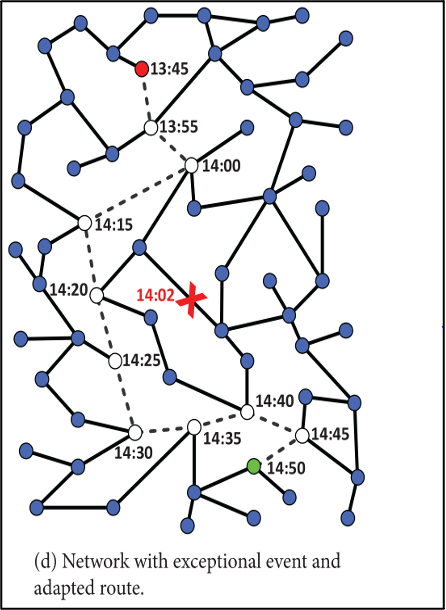
\includegraphics{figures/fig1.png}

}

\caption{Figure 1: Within-day replanning approach for a MATSim routing
problem.}

\end{figure}

While iterative systems leverage best-response modules, within-day
systems necessitate using a best-guess module. This approach means that
travel times can be optimized to a stable state with an iterative
approach, but this is not the case with a within-day approach. An
inherent attribute of within-day replanning is that it doesn't converge
to a user equilibrium, unlike an iterative process. Decisions, appearing
optimal in the heat of the moment, often reveal themselves as suboptimal
upon retrospective evaluation. Given the limited information available
to the agents in a within-day system, they may not necessarily choose
the path with the shortest travel time post-incident, as discussed by
Dobler in 2016.

Replanning contains two categories: replanning an element of the
activity and executing the replanned elements. Elements include the
start and end times of the trip, the trip's location, route, mode
choice, or the dropping of a trip entirely. The system can execute plans
for in-the-moment events or those performed in the future. In a
presently performed procedure, we cannot conduct all replanning actions
(e.g., we can no longer alter the start time of an activity or the
transport mode of a trip currently being performed) (Dobler and Nagel
2016). Figure 2: Iterative and within-day replanning MATSim loop.
illustrates where within-day replanning fits within a MATSim loop.

\begin{figure}

{\centering 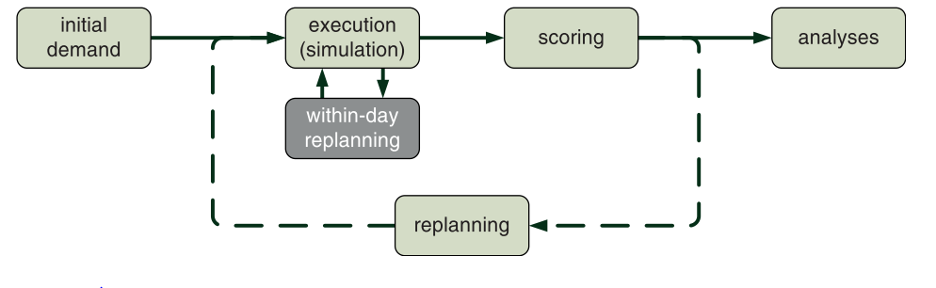
\includegraphics{figures/fig2.png}

}

\caption{Figure 2: Iterative and within-day replanning MATSim loop.}

\end{figure}

An alternative to iterative or within-day replanning only approaches is
to combine them. For example, we cannot plan situations like parking or
car-sharing thoroughly, requiring iterative and within-day replanning
methods. An agent can arrange a parking activity but cannot predict
which parking spots will be available when they arrive. Thus, we use
within-day replanning when the agent starts their parking choice.

In general, within-day or en-route replanning means that travelers
replan during the day or on their route, which means that the simulation
needs to influence the agent while the network is running.
(\textbf{dobler2016explains?}) that we influence agents' decisions
through loops or by having users' routes dependent on the next link that
they choose. Because going through all links and nodes at every step
would be computationally challenging, we may set certain links to be
non- active and removed from the computation (Dobler and Nagel 2016).
The two implementation methods Dobler described are plan-based
implementation and replacing the agent.

In a plan-based implementation, a loop is used where each agent has the
chance to deliberate in every time step. The agent can decide that they
have nothing to deliberate and return immediately. Because the number of
links is typically much smaller than the number of agents in a scenario,
massive optimization is necessary to make the loop computationally
efficient. For this reason, we could ask each agent to choose a link
only when they need to make a decision.

Such event-driven planning requires the agents to be re-programmed to
have enough capabilities to be oriented about themselves (i.e., be able
to compute plausible routes). Agents will only need to perform such
computation when replanning is triggered by an event like an emergency
warning or unexpected congestion; otherwise, they will follow their
usual daily plans.

Re-programing agents and implementing within-day replanning, as shown in
Figure 2: Iterative and within-day replanning MATSim loop., requires the
implantation of a \emph{MobsimEngine}, which can be plugged into the
mobility simulator seen in the execution phase of Figure 2: Iterative
and within-day replanning MATSim loop (Axhausen, Horni, and Nagel
2016-08-10, 2016-08). Dobler and Nagel (2016) describes it this way,
``in every simulated time step, the QSim iterates over all registered
\emph{MobsimEngines} and allows them to simulate the current time step.
Besides simulation of the traffic flows, those engines can also let
agents start or end activities'' (Dobler and Nagel 2016, 193). The
engines contain within-day replanning logic called
\emph{WithinDayEngine}, which helps track agents and adapt their plans
(Dobler and Nagel 2016). Not all agents need to compute plausible routes
at every turn, so an \emph{AgentSelector} is used to select the agents
to be replanned. \emph{AgentFilters} assist them in narrowing the search
population (Dobler and Nagel 2016). Lastly, \emph{TravelTimeCollectors}
are part of the \emph{WithinDayEngine} and provide actual link travel
times to the replanners by collecting and averaging travel times of
agents that have recently passed a link during a given time (Dobler and
Nagel 2016). The elements described above make up the plan-based system.

A significant incident modeling, plan-based system study used MATSim to
simulate traffic incidents (Kaddoura and Nagel 2018-01-01, 2018-01).
Their research explains that MATSim models transport users as individual
agents. MATSim is iterative and allows users to adjust travel plans
during a single iteration, from iteration to iteration, or both
(Kaddoura and Nagel 2018-01-01, 2018-01). Kaddoura and Nagel accessed
their incident data via the HERE application programming interface for
traffic incidents. This incident data included Traffic Message Channel
(TMC) information indicating an incident's cause and severity. With such
robust data, Kaddoura and Nagel could categorize incidents as long or
short-term and model each accordingly in MATSim. Long-term effects
include multiple-day lane closures, whereas short-term incidents affect
transport supply for less than a day. Their simulation was based on an
inner-city network in Berlin, Germany. Figure 3: Traffic incidents
mapped on the Berlin network illustrates the type of incidents modeled
and their severity. In this example, a crash on the southern inner-city
motorway ring road led to a full road closure, and several construction
sites caused partial capacity reductions.

\begin{figure}

{\centering 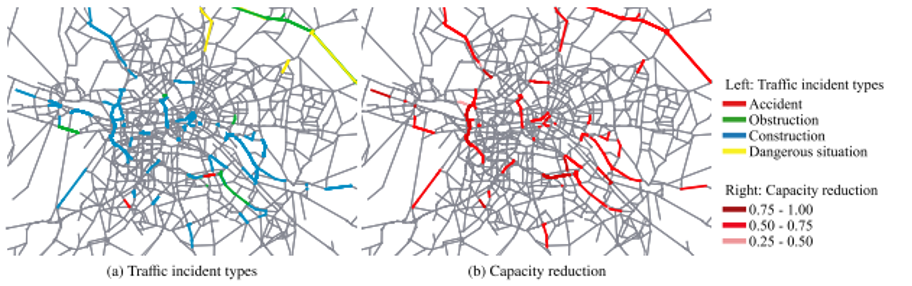
\includegraphics{figures/fig3.png}

}

\caption{Figure 3: Traffic incidents mapped on the Berlin network.}

\end{figure}

Kaddoura and Nagel (2018-01-01, 2018-01) found that long-term traffic
incidents increase traffic congestion and the average car travel time by
313 sec (+18\%) per trip. Short-term traffic incidents increase the
average travel time per car trip by another 136 sec (+8\%).
Additionally, they found that for 44\% of all car trips, the agent's
transport route contained at least one road segment for which the
capacity or speed limit was reduced because of an incident. Their study
concluded that networks in which transport users had high levels of
knowledge about the incidents and resulting traffic congestion still
experienced an increase in travel time caused by long and short-term
incidents. Finally, Kaddoura and Nagel asserted that ``accounting for
traffic incidents makes the model more realistic, allowing for an
improved policy investigation'' (Kaddoura and Nagel 2018-01-01, 2018-01,
885). The modeling performed by Kaddoura and Nagel is just one example
of research on MATSim's capacity for incident-based simulations.

A MATSim model developed by Li and Ferguson (2020-01-01, 2020-01)
included a range of rescheduling options, such as departure time, mode
choice, and trip cancellation. Their simulation found that if travelers
received notice of an incident, they would either depart early from
their place of origin or switch to public transport (Li and Ferguson
2020-01-01, 2020-01). The process proposed by Li and Ferguson is
beneficial because it allows agents to reassess their mode choice or
route assignment based on the notice of a reported incident. Li and
Ferguson show that users care about total travel time and travel time
variability (risk tolerance to a certain degree). The receiving of
notifications about incidents by agents impacted both factors. They
concluded that ``the provision of real-time traffic information is a
useful approach to mitigating the side-effects of incidents through
helping transport users efficiently adapt their day plans'' (Li and
Ferguson 2020-01-01, 2020-01, 96).

Additionally, they found that ``most of the travelers notified of being
affected by incidents are simulated to depart early or switch to public
transport, which effectively reduces the average travel time delay
caused by disruptions'' (Li and Ferguson 2020-01-01, 2020-01, 96). Their
findings validate the conclusions of @sisiopiku2007 that making incident
information available to agents leads to decreases in travel time and
congestion. Like the studies already mentioned, there have been various
modifications to and research on MATSim and its capacity.

In Thailand's capital, Bangkok, a study conducted by Peungnumsai et al.
(2019) demonstrated the potency of the MATSim framework in portraying
the impact of rush hour congestion on select traffic links. Peungnumsai
ran various simulation iterations, loading the selected links with a
different number of agents: 10, 100, and 500. The data collected and the
subsequent analysis substantiated MATSim's capability to demonstrate the
congestion-induced variations in travel time. Furthermore, it was
observed that as the number of agents in the simulation increased, there
was a proportional surge in computing time, physical memory usage, and
the size of the output file. Despite the scale of these simulations
being relatively small, MATSim has the capacity to simulate up to 10-100
million agents, encompassing various modes of transportation like
bicycles, motorbikes, cars, buses, and taxis (Peungnumsai et al. 2019).

In a contrasting study conducted in Copenhagen, Denmark, Paulsen,
Rasmussen, and Nielsen (2018) utilized MATSim to contrast the
reliability of automobile and railway travel times. His methodology
involved using an extension of MATSim centered around an event-based
public transport router, which facilitates optimal route selection for
public transport users by comparing the effectiveness of routes over
several iterations. Paulsen's simulation of travel times for both cars
and trains yielded an interesting finding: passenger delays were
significantly influenced by the adaptiveness of their chosen routes.
However, he noted that passenger travel times tended to be more
unpredictable than trains, and this unpredictability escalated with the
degree of route adaptiveness. He concluded that the adaptiveness of
route selection contributed to significant travel time fluctuations, a
conclusion that aligns with the findings of Li and Ferguson (2020-01-01,
2020-01).

In essence, the studies encapsulated in Section 2.3 validate the
effectiveness of the open-source software MATSim, in simulating traffic
incidents, congestion, and travel times. This evidence accentuates how
the proper application of MATSim or similar Dynamic Traffic Assignment
(DTA) models can account for traffic incidents, thereby enhancing the
realism of the models. This type of model, in turn, can facilitate more
effective policy investigation, as noted by Kaddoura and Nagel
(2018-01-01, 2018-01).

\hypertarget{summary}{%
\section{Summary}\label{summary}}

As explained in this section there has been extensive research into IMT
effectiveness and its ability to restore traffic flow following long-
and short-term disturbances. Additionally, several studies have examined
how to effectively model traffic incidents and show their impact on
travel time, congestion, and mode choice. However, in these vast arrays
of findings, there is a gap in research on modeling IMT effectiveness
and incident impact on a loaded with realistic agents. As a result, it
is difficult for researchers to understand how changes to incident
generation or to IMT availability may impact traffic conditions, for
good or for bad. In this research, we seek to bring these two strands
together, attempting to model incident response in a microsimulation
framework to bring realism and detail to the IMT deployment question.

\bookmarksetup{startatroot}

\hypertarget{methodology}{%
\chapter{Methodology}\label{methodology}}

\hypertarget{incident-response-in-matsim}{%
\subsection{3.1 Incident Response in
MATSim}\label{incident-response-in-matsim}}

This section of the methodology outlines the development of the model
for the Utah IMT Optimization project. As stated in sections 2.2 and 2.3
of the literature review, the model is designed to effectively
demonstrate the effects of traffic incidents on the overall traffic
flow, and the subsequent influence of Incident Management Teams (IMTs)
when integrated into the model.

We explain how incidents and IMT vehicles are represented within the
MATSim model and discuss several adjustments made to the behavior of
MATSim agents within the model configuration. Our approach to incident
modeling primarily draws from and expands on the research of
(\textbf{kaddoura2016?}). For a more detailed understanding, refer to
The Multi-Agent Transport Simulation (MATSim) textbook.

\hypertarget{network-change-events}{%
\subsubsection{3.1.1 Network Change
Events}\label{network-change-events}}

Each link in a MATSim network possesses specific attributes, such as
link type, length, number of lanes, free-flow speed, and capacity. To
simulate unexpected events, it's essential to adjust one or more of
these parameters at a specific time during the simulation. The capacity
to modify a network, as referred to in the MATSim textbook, is known as
a Time-Dependent Network, and unforeseen incidents or any factors that
alter the network's characteristics are termed Network Change Events
(NCEs).

Section 6.1 of the MATSim textbook outlines how to adapt the parameters
of a MATSim configuration file to allow for time-variant network
attributes and how to implement network change events. These events can
modify a link's free-flow speed, number of lanes, or capacity. To
activate a network change event, the system needs to know the time of
the event (startTime), the affected link(s) (link refID), the nature of
the change (free-flow speed, lanes, or capacity), and the specific value
of the change.

Within the context of the Utah IMT optimization problem, changes are
triggered when an incident is reported and when an IMT arrives at the
affected link. These changes will influence the link's capacity based on
the incident data, which will be discussed in more detail in section
3.2.3. Unlike (\textbf{kaddoura2016?})'s work, this study does not
consider long-term capacity reduction events such as road construction,
focusing solely on short-term incidents like accidents or vehicle
breakdowns. The diminished capacity of a specific link would typically
affect both regular agents (those included in the baseline simulation
scenario) and IMT agent vehicles. If a subnetwork is utilized, IMT
trucks, similar to other emergency vehicles like ambulances and
firetrucks, would be less affected by congestion caused by daily traffic
or unexpected incidents.

The implementation of the MATSim within-day replanning module plays a
significant role in the rerouting of other agents on the road after an
incident.

\hypertarget{within-day-replanning}{%
\subsubsection{3.1.2 Within-Day
Replanning}\label{within-day-replanning}}

\textless\textless{} The concept of within-day replanning is applied to
a certain extent in the model, as detailed in Chapter 30 of the MATSim
textbook. However, I plan to delve deeper into this concept to ensure
its correct application within our study. Subsequently, I will refine
the wording of this section to accurately convey its implementation
within our model. \textgreater\textgreater{}

\hypertarget{vehicle-assignment}{%
\subsubsection{3.1.3 Vehicle Assignment}\label{vehicle-assignment}}

When an incident occurs within the MATSim simulation, one or more
Incident Management Team (IMT) vehicles are dispatched to manage the
situation. A dispatch algorithm determines the most suitable vehicle for
the task. The model can select the IMT unit(s) based either on a
least-cost path calculation that factors in congestion and link speed or
the shortest path between the vehicle's location and the incident site.
The chosen method will partially depend on how swiftly the IMT units can
navigate through traffic. If a subnetwork is utilized, the IMT trucks
would be less affected by congestion and free-flow speed, potentially
making the shortest path calculation more suitable. Conversely, if an
IMT moves through traffic like a standard vehicle, using a least-cost
path calculator within the simulation would likely be the preferred
option.

In the context of this project, the Utah IMT system operates in tandem
with the Utah Highway Patrol system under the same dispatch service.
IMTs in Utah are equipped with sirens and flashing lights similar to
those on a highway patrol vehicle, and they operate within specific
zones. For instance, there are multiple zones in Salt Lake and Davis
Counties where IMT vehicles are distributed. Given that IMTs can
navigate traffic like other emergency vehicles, the Utah Highway Patrol
dispatch requests the nearest available vehicle(s) to respond to an
incident when it occurs. It's worth noting that due to limited
resources, an incident ideally requiring assistance from 2 or 3 IMT
units may only receive one vehicle, potentially leading to longer
management or cleanup times.

\hypertarget{incident-response}{%
\subsubsection{3.1.4 Incident Response}\label{incident-response}}

As discussed in Section 3.1.1, a critical element in simulating the
effects of incidents on agents within the MATSim network is Network
Change Events (NCEs). This mechanism, which illustrates how incidents
can impact user behavior, will also be used to demonstrate how the
reactions of IMTs influence agents' travel times and paths.

Once the vehicle assignment algorithm dispatches one or more IMT units
to an incident, a decision must be made on what percentage of the
incident link's capacity is restored upon the IMT's arrival. An arriving
IMT can either hasten the restoration of the capacity to normal levels
or enhance the capacity by a certain percentage `X.' These adjustments
hinge on the available incident data and findings from other research
regarding IMT effectiveness.

Kim et al. (2012-04-01, 2012-04) discusses the cost-benefit ratio of
different IMT fleet sizes, and other studies have attempted to gauge the
duration of an incident's impact without an IMT and contrast that with
the length of time that an incident affects traffic when an IMT is
dispatched. Given the correct information or building upon certain
assumptions, one can establish a capacity restoration factor to be
applied upon a vehicle's arrival at an incident site.

Figure 4 below provides a potential example of how an incident, with no
IMT response, might affect a network in comparison to scenarios where
one IMT responds, followed by the response of a secondary unit.

\begin{figure}

{\centering 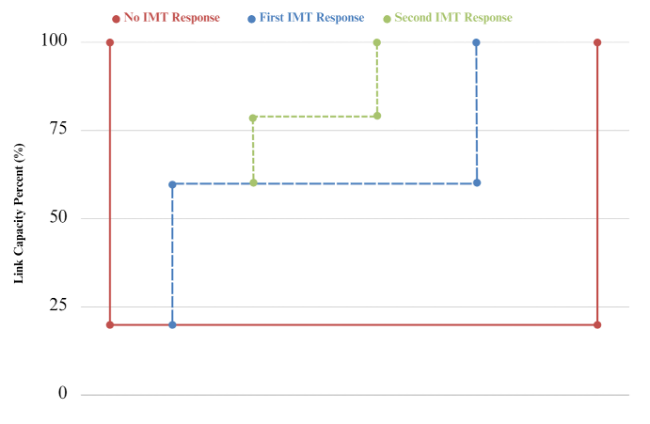
\includegraphics{figures/fig4.png}

}

\caption{Figure 4: Changes upon arrival.}

\end{figure}

\hypertarget{simulation-scenarios}{%
\subsection{3.2 Simulation Scenarios}\label{simulation-scenarios}}

Loading incidents and IMT response vehicles into the Utah Optimization
model is a significant aspect of this project's methodology. Another
crucial element involves running scenarios to quantify the impact of
both incidents and IMT arrivals. Various factors influence these
quantitative comparisons. These include the type of network and plans
files used during the simulation, the processed and selected incident
data, and the locations and quantities of IMT vehicles included in the
simulations. Each of these components builds on prior research related
to IMTs in Utah, MATSim studies on Demand Responsive Transport (DRT),
and transportation modeling research conducted by the Wasatch Front
Regional Council in various traffic modeling projects throughout Utah.

\hypertarget{wasatch-front-base-scenario}{%
\subsubsection{3.2.1 Wasatch Front Base
Scenario}\label{wasatch-front-base-scenario}}

In this section, we aim to outline the origins of the network and plans
file and their usage in other research conducted by the Wasatch Front
Regional Council (WFRC).

\textless\textless{} Dr.~Macfarlane has provided information about the
source of these plans. I will review his notes before expanding this
section. \textgreater\textgreater{}

The network and plans have been calibrated and represent a typical day's
traffic in the regions where most IMT vehicles operate.

\hypertarget{incident-imt-scenario}{%
\subsubsection{3.2.2 Incident \& IMT
Scenario}\label{incident-imt-scenario}}

We will detail the variety of scenarios we executed in this section,
specifying the types based on the number of incidents and the quantity
of Incident Management Teams (IMTs) involved. We'll clarify why we chose
to execute the specific number of tests and scenarios.

\textless\textless{} Brynn has prepared a table detailing these
different scenario types, which we could include here if desired.
\textgreater\textgreater{}

Essentially, we have six scenarios:

1. A baseline with no IMTs.

2. A baseline with no IMTs and increased incident frequency.

3. Current IMT resources with current incident frequency.

4. Current IMT resources with increased incident frequency.

5. Improved (added) IMT resources with the current frequency of
incidents.

6. Improved IMT resources with increased frequency of incidents.

Our goal is to run at least ten days of simulations for each scenario.

\hypertarget{incident-data}{%
\subsubsection{3.2.3 Incident Data}\label{incident-data}}

\textless\textless{} TO DO: summarize the methodology used by Joel Hyer
and to describe where our incident data came from
\textgreater\textgreater{}

\hypertarget{incident-sampling}{%
\subsubsection{3.2.4 Incident Sampling}\label{incident-sampling}}

In order to determine how many incidents should be modeled in a given
day, representing current incident frequency, we performed an analysis
on the incident data we received to create a distribution of incident
count frequency to sample from.

We wrote code using Pandas in Python to read data into a data frame,
remove duplicate entries, and manipulate the `Call Received Time' and
`Call Type' columns. The data frame is then grouped by date and call
type to count incidents. The result is a new data frame showing incident
frequency per day. These frequencies are used to create a weighted
distribution for sampling. Using a random seed value, to ensure
reproducibility, the code performs random sampling by selecting ten days
from the distribution of incident numbers based on the calculated
frequencies. The sample results in ten values that will be used in
MATSim to determine how many incidents to generate in the simulation for
ten different scenarios.

For our increased frequency scenarios, we aimed to assess the impact of
a significant surge in daily incidents on the IMT system. To achieve
this, we used the higher end of the 2022 data as a reference, which
included one day with 21 incidents, one day with 20 incidents, two days
with 19 incidents, and two days with 18 incidents. This approach allowed
us to test the effectiveness and coverage of the IMT program under more
extreme demand. Because this collection is only representative of 6
days, we included one additional day of each incident count, choosing to
simulate two days with 21 incidents, two days with 20 incidents, three
days with 19 incidents, and three days with 18 incidents.

\begin{figure}

{\centering 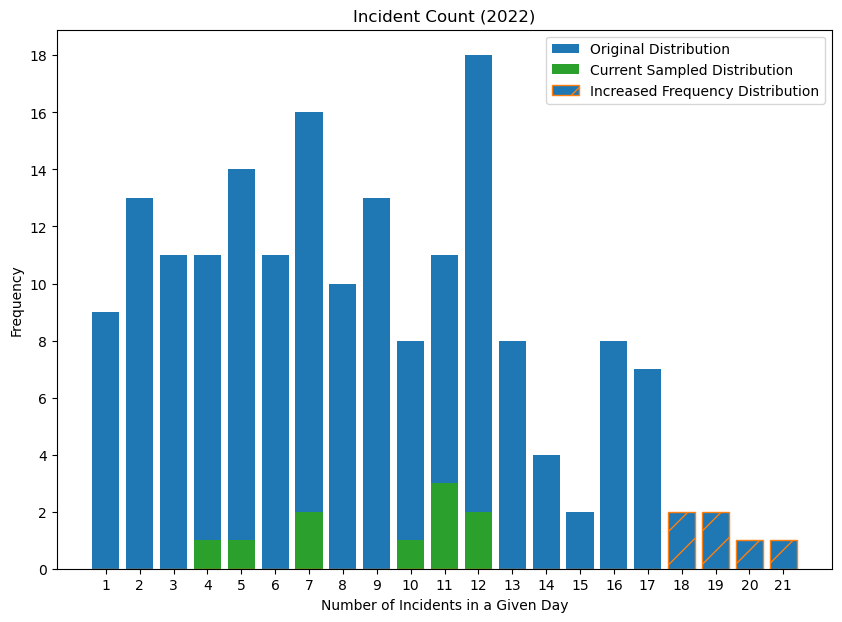
\includegraphics{figures/fig5.png}

}

\caption{Figure 5: Incident Sampling.}

\end{figure}

\bookmarksetup{startatroot}

\hypertarget{applications}{%
\chapter{Applications}\label{applications}}

This section might be called ``Results'' instead of ``Applications,''
depending on what it is that you are working on. But you'll probably say
something like ``The initial model estimation results are given in
Table~\ref{tbl-estimationresults}'' That table is created with the
\texttt{modelsummary()} package and function.

\hypertarget{tbl-estimationresults}{}
\begin{table}
\caption{\label{tbl-estimationresults}Model Summary Results }\tabularnewline

\centering
\begin{tabular}[t]{lcc}
\toprule
  & Model 1 & Model 2\\
\midrule
typesportuv & 0.833 (5.945) & 0.815 (5.805)\\
 & (0.140) & (0.140)\\
typesportcar & 0.614 (4.192) & 0.628 (4.259)\\
 & (0.146) & (0.147)\\
typestwagon & -1.415 (-22.979) & -1.428 (-23.119)\\
 & (0.062) & (0.062)\\
typetruck & -1.002 (-20.600) & -1.010 (-20.673)\\
 & (0.049) & (0.049)\\
typevan & -0.812 (-17.431) & -0.806 (-17.183)\\
 & (0.047) & (0.047)\\
price & -0.221 (-8.475) & -0.191 (-7.130)\\
 & (0.026) & (0.027)\\
range &  & 0.003 (18.923)\\
 &  & (0.000)\\
\midrule
Num.Obs. & 27924 & 27924\\
AIC & 15460.9 & 15075.0\\
RMSE & 0.80 & 0.78\\
\bottomrule
\end{tabular}
\end{table}

Sometimes, it is nice to put the models or your other results into a
figure instead of a table. Have a look at Figure~\ref{fig-modelplot}.
Note that your figures might look better in pdf if you use the
\texttt{tikz} rendering device.

\begin{figure}

{\centering 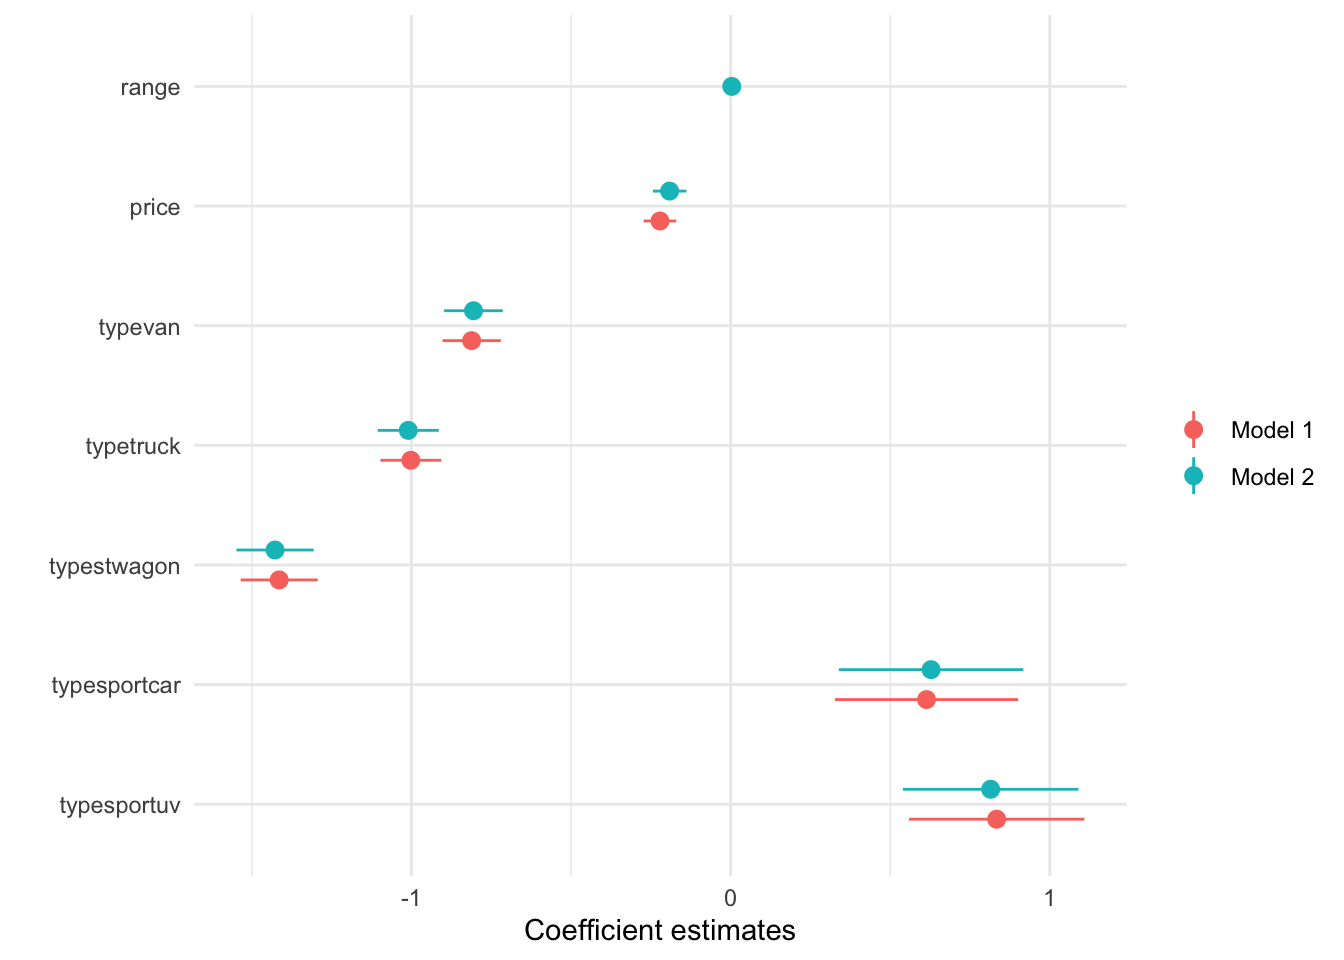
\includegraphics{04_results_files/figure-pdf/fig-modelplot-1.pdf}

}

\caption{\label{fig-modelplot}Estimated model coefficients and
confidence intervals.}

\end{figure}

With those results presented, you can go into a discussion of what they
mean. first, discuss the actual results that are shown in the table, and
then any interesting or unintuitive observations.

\hypertarget{additional-analysis}{%
\section{Additional Analysis}\label{additional-analysis}}

Usually, it is good to use your model for something.

\begin{itemize}
\tightlist
\item
  Hypothetical policy analysis
\item
  Statistical validation effort
\item
  Equity or impact analysis
\end{itemize}

If the analysis is substantial, it might become its own top-level
section.

\bookmarksetup{startatroot}

\hypertarget{conclusions}{%
\chapter{Conclusions}\label{conclusions}}

This section need not be overly long. You should address any limitations
of your results, such as dependence on underlying assumptions or
geographic scope. You should also provide a map for future research.

Finally, you should underline the contributions of this work and any
practical relevance.

\bookmarksetup{startatroot}

\hypertarget{references}{%
\chapter*{References}\label{references}}
\addcontentsline{toc}{chapter}{References}

\markboth{References}{References}

\hypertarget{refs}{}
\begin{CSLReferences}{1}{0}
\leavevmode\vadjust pre{\hypertarget{ref-axhausen2016}{}}%
Axhausen, Kay W., Andreas Horni, and Kai Nagel. 2016-08-10, 2016-08.
\emph{The Multi-Agent Transport Simulation {MATSim}}. {Ubiquity Press}.

\leavevmode\vadjust pre{\hypertarget{ref-bivina2016}{}}%
Bivina, G. R., Vishrut Landge, and V. S. Sanjay Kumar. 2016-01-01,
2016-01. {``Socio Economic Valuation of Traffic Delays.''}
\emph{Transportation Research Procedia}, International conference on
transportation planning and implementation methodologies for developing
countries (12th {TPMDC}) selected proceedings, {IIT} bombay, mumbai,
india, 10-12 december 2014, 17 (2016-01-01, 2016-01): 513--20.
\url{https://doi.org/10.1016/j.trpro.2016.11.104}.

\leavevmode\vadjust pre{\hypertarget{ref-boyles2018}{}}%
Boyles, Stephen. 2018-01-22, 2018-01. {``Introduction to Dynamic Traffic
Assignment,''} 2018-01-22, 2018-01.

\leavevmode\vadjust pre{\hypertarget{ref-dobler2016}{}}%
Dobler, Christoph, and Kai Nagel. 2016. {``Within-Day Replanning.''} In.
{Ubiquity Press}.

\leavevmode\vadjust pre{\hypertarget{ref-kaddoura2018}{}}%
Kaddoura, Ihab, and Kai Nagel. 2018-01-01, 2018-01. {``Using Real-World
Traffic Incident Data in Transport Modeling.''} \emph{Procedia Computer
Science}, The 9th international conference on ambient systems, networks
and technologies ({ANT} 2018) / the 8th international conference on
sustainable energy information technology ({SEIT-2018}) / affiliated
workshops, 130 (2018-01-01, 2018-01): 880--85.
\url{https://doi.org/10.1016/j.procs.2018.04.084}.

\leavevmode\vadjust pre{\hypertarget{ref-kim2012}{}}%
Kim, Woon, Mark Franz, Gang-Len Chang, and Md.). Dept. of Civil and
Environmental Engineering University of Maryland (College Park.
2012-04-01, 2012-04. {``Enhancement of Freeway Incident Traffic
Management and Resulting Benefits.''}

\leavevmode\vadjust pre{\hypertarget{ref-li2020}{}}%
Li, Jingsi, and Neil Ferguson. 2020-01-01, 2020-01. {``A
Multi-Dimensional Rescheduling Model in Disrupted Transport Network
Using Rule-Based Decision Making.''} \emph{Procedia Computer Science},
The 11th international conference on ambient systems, networks and
technologies ({ANT}) / the 3rd international conference on emerging data
and industry 4.0 ({EDI40}) / affiliated workshops, 170 (2020-01-01,
2020-01): 90--97. \url{https://doi.org/10.1016/j.procs.2020.03.012}.

\leavevmode\vadjust pre{\hypertarget{ref-ozbay2013}{}}%
Ozbay, Kaan, Cem Iyigun, Melike Baykal-Gursoy, and Weihua Xiao.
2013-03-01, 2013-03. {``Probabilistic Programming Models for Traffic
Incident Management Operations Planning.''} \emph{Annals of Operations
Research} 203 (1): 389--406.
\url{https://doi.org/10.1007/s10479-012-1174-6}.

\leavevmode\vadjust pre{\hypertarget{ref-pal2002}{}}%
Pal, R., and K. C. Sinha. 2002. {``{SIMULATION MODEL FOR EVALUATING AND
IMPROVING EFFECTIVENESS OF FREEWAY SERVICE PATROL PROGRAMS}.''}
\emph{Journal of Transportation Engineering} 128 (4).

\leavevmode\vadjust pre{\hypertarget{ref-paulsen2018}{}}%
Paulsen, Mads, Thomas Kjær Rasmussen, and Otto Anker Nielsen. 2018.
{``Modelling Railway-Induced Passenger Delays in Multi-Modal Public
Transport Networks: {An} Agent-Based Copenhagen Case Study Using
Empirical Train Delay Data: 14th Conference on Advanced Systems in
Public Transport and {TransitData} 2018.''} In.

\leavevmode\vadjust pre{\hypertarget{ref-peungnumsai2019}{}}%
Peungnumsai, Apantri, Hiroyuki Miyazaki, Apichon Witayangkurn, and
Masanobu Kii. 2019. {``A Review of {MATSim}: {A} Pilot Study of
Chatuchak, Bangkok.''}

\leavevmode\vadjust pre{\hypertarget{ref-schultz2019}{}}%
Schultz, Grant G., Mitsuru Saito, Dennis L. Eggett, Logan S Bennett,
Mitchell G Hadfield, Brigham Young University. Dept. of Civil, and
Environmental Engineering. 2019-04-01, 2019-04. {``Analysis of
Performance Measures of Traffic Incident Management in Utah.''}

\leavevmode\vadjust pre{\hypertarget{ref-skabardonis1998}{}}%
Skabardonis, Alexander. 1998. {``Evaluation of the Freeway Service
Patrol ({FSP}) in Los Angeles.''} \emph{PATH Research Report}.

\leavevmode\vadjust pre{\hypertarget{ref-vanlint2012}{}}%
van Lint, Hans, Onno Miete, Henk Taale, and Serge Hoogendoorn.
2012-01-01, 2012-01. {``Systematic Framework for Assessing Traffic
Measures and Policies on Reliability of Traffic Operations and Travel
Time.''} \emph{Transportation Research Record} 2302 (1): 92--101.
\url{https://doi.org/10.3141/2302-10}.

\leavevmode\vadjust pre{\hypertarget{ref-wirtz2005}{}}%
Wirtz, John J., Joseph L. Schofer, and David F. Schulz. 2005-01-01,
2005-01. {``Using Simulation to Test Traffic Incident Management
Strategies: {The} Benefits of Preplanning.''} \emph{Transportation
Research Record} 1923 (1): 82--90.
\url{https://doi.org/10.1177/0361198105192300109}.

\end{CSLReferences}



\end{document}
